\documentclass[
	letterpaper, % Paper size, specify a4paper (A4) or letterpaper (US letter)
	10pt, % Default font size, specify 10pt, 11pt or 12pt
]{CSUniSchoolLabReport}

%----------------------------------------------------------------------------------------
%	REPORT INFORMATION
%----------------------------------------------------------------------------------------

\title{Lab Two\\ Power Systems Analysis \\ EECE5682} % Report title

\author{Michael \textsc{Brodskiy}\\ \small \href{mailto:Brodskiy.M@Northeastern.edu}{Brodskiy.M@Northeastern.edu}}

\date{October 17, 2024} % Date of the report

%----------------------------------------------------------------------------------------


\begin{document}

\maketitle % Insert the title, author and date using the information specified above

\begin{center}
	\begin{tabular}{l r}
		Date Performed: & \today \\ % Date the experiment was performed
		Instructor: & Professor \textsc{Abur} \\ % Instructor/supervisor
	\end{tabular}
\end{center}

\newpage

\begin{abstract}

  This laboratory experiment explores the transmission line model via integration through SimuLink. Concepts explored include the impedance of a transmission line, series capacitance, and shunt capacitance.

\end{abstract}

\begin{flushleft}

  \textsc{Keywords:} \underline{transmission line}, \underline{model}, \underline{SimuLink}, \underline{line impedance}, \underline{series capacitance}, \underline{shunt capacitance}

\end{flushleft}

\newpage

\section{Introduction \& Objectives}

This experiment begins by integrating the following diagram into MATLAB's SimuLink environment:

\begin{figure}[H]
  \centering
  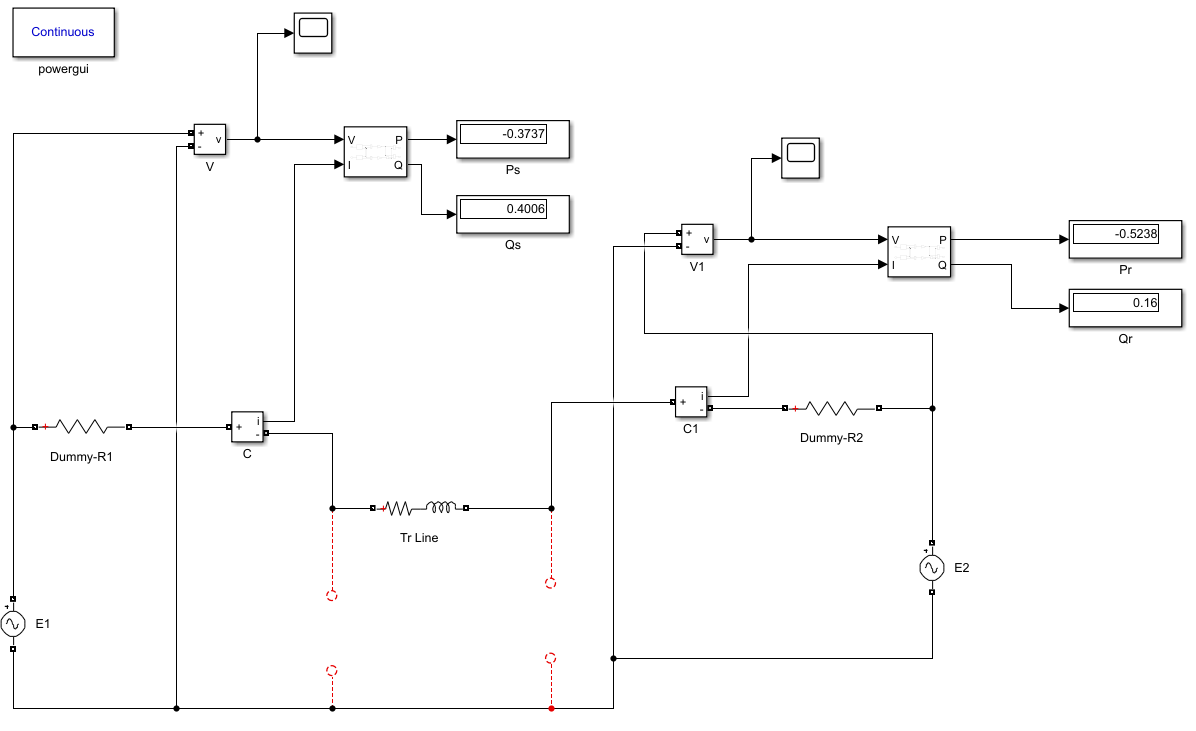
\includegraphics[width=.9\textwidth]{Figures/Lab\ Three/L3ABCE.png}
  \caption{Simulated Circuit (No Capacitors or Series Capacitor)}
  \label{fig:1}
\end{figure}

This circuit was used for parts A, B, C, and E. Note that, when it was specified to add a series capacitor, the reactance of the transmission line ($.5+1.2j\to.5+.8j$) was modified, instead of adding a new capacitor in series. For part D, the following circuit was simulated:

\begin{figure}[H]
  \centering
  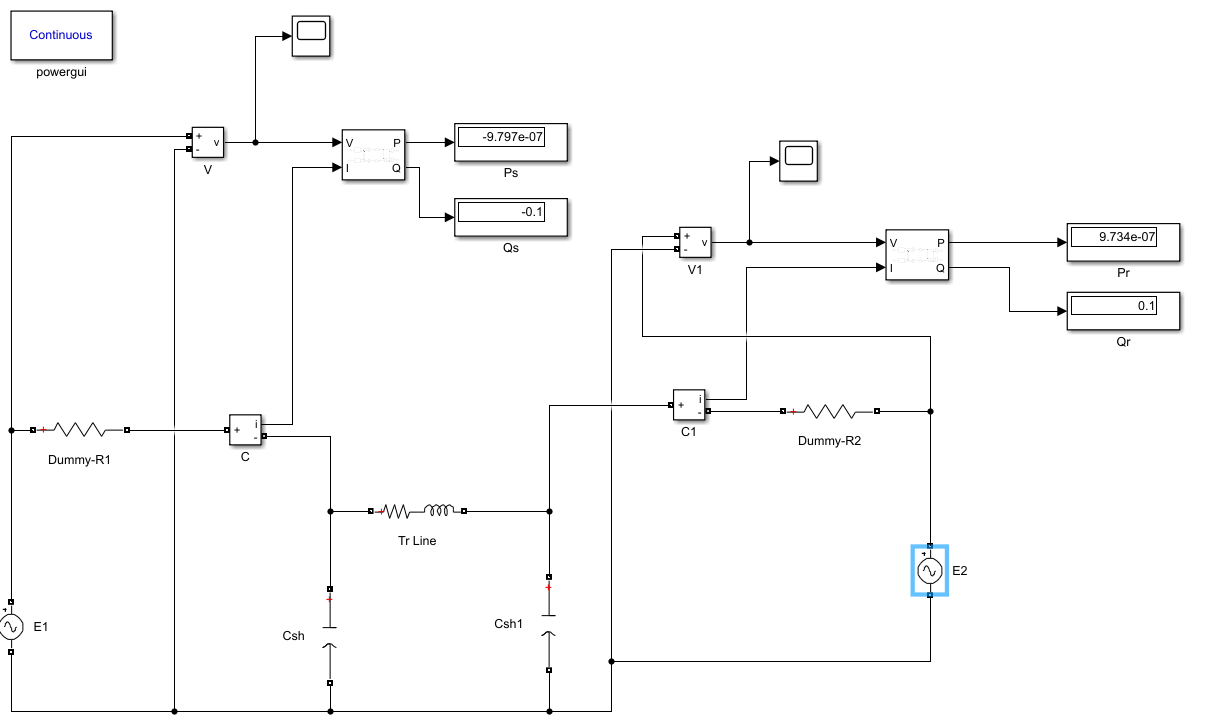
\includegraphics[width=.9\textwidth]{Figures/Lab\ Three/L3D.png}
  \caption{Simulated Circuit (Shunt Capacitors)}
  \label{fig:2}
\end{figure}


\section{Results \& Analysis} 

\subsection{Parts A \& B: Simulating with No Capacitors}

Simulating the circuit shown in Figure \ref{fig:1} allowed us to obtain the following table:

\begin{center}
  \begin{tabular}[H]{|c|c|c|}
    \hline
    $P_{12}[p.u.]$ & $P_{21}[p.u.]$ & $\theta_2[^{\circ}]$\\
    \hline
    0 & 0 & 0\\
    \hline
    .3941 & .3152 & -30\\
    \hline
    .7612 & .4673 & -60\\
    \hline
    1.004 & .4146 & -90\\
    \hline
    \cellcolor{green} 1.059 & .1714 & -120\\
    \hline
    .9075 & -.1975 & -150\\
    \hline
    .5928 & -.5928 & -180\\
    \hline
    .1978 & -.9069 & -210\\
    \hline
    -.1695 & \cellcolor{red} -1.058 & -240\\
    \hline
    -.4124 & -1.004 & -270\\
    \hline
    -.4657 & -.7611 & -300\\
    \hline
    -.3144 & -.394 & -330\\
    \hline
    0 & 0 & -360\\
    \hline
  \end{tabular}
\end{center}

We may observe (in green) that $P_{12}$ is maximized when $\theta_2=-120[^{\circ}]$, with a maximum value of $P_{12}=1.059[p.u.]$. Furthermore, we may observe that $-P_{21}$ is maximized (in red) when $\theta_2=-240[^{\circ}]$, with a maximum value of $-P_{21}=1.058[p.u.]$. It may be observed that the two maximum values are the same (with a slight margin caused by simulation imperfections).

\subsection{Part C: Series Capacitor}

As stated above, a series capacitor was introduced in this scenario. This was done by modifying the transmission line from $.5+1.2j$ to $.5+.8j$ per-unit impedance. Simulating the circuit allowed us to obtain the following data:

\begin{center}
  \begin{tabular}[H]{|c|c|c|}
    \hline
    $P_{12}[p.u.]$ & $P_{21}[p.u.]$ & $\theta_2[^{\circ}]$\\
    \hline
    0 & 0 & 0\\
    \hline
    .5239 & .374 & -30\\
    \hline
    1.058 & .4983 & -60\\
    \hline
    1.459 & .3394 & -90\\
    \hline
    \cellcolor{green} 1.62  & -.06226 & -120\\
    \hline
    1.498 & -.5989 & -150\\
    \hline
    1.125 & -1.125 & -180\\
    \hline
    .6002 & -1.498 & -210\\
    \hline
    .06387 & \cellcolor{red} -1.619 & -240\\
    \hline
    -.3361 & -1.459 & -270\\
    \hline
    -.4969 & -1.058 & -300\\
    \hline
    -.3737 & -.5238 & -330\\
    \hline
    0 & 0 & -360\\
    \hline
  \end{tabular}
\end{center}

We may observe that the maximum values once again occur at $120\left[ ^{\circ} \right]$ and $240\left[ ^{\circ} \right]$ for $P_{12}$ and $-P_{21}$, respectively. Once again, $P_{12}=1.62[p.u.]\approx -P_{21}$; however, we may observe that the magnitude of the power has increased in comparison to Parts A and B. Thus, we may conclude that adding a capacitor in series may help with increasing the real power transmission. This allows for better control of (and increased) voltage and improved system stability. A drawback, however, is that a series-compensated line would produce resonance frequencies at lower frequencies than those produced by the power.

\subsection{Part D: Shunt Capacitors}

We now remove the series compensation and add in shunt capacitors, as shown in Figure \ref{fig:2}. This allows us to obtain the following data:

\begin{center}
  \begin{tabular}[H]{|c|c|c|}
    \hline
    $P_{12}[p.u.]$ & $P_{21}[p.u.]$ & $\theta_2[^{\circ}]$\\
    \hline
    0 & 0 & 0\\
    \hline
    .3946 & .3154 & -30\\
    \hline
    .7628 & .467 & -60\\
    \hline
    1.006 & .4143 & -90\\
    \hline
    1.058  & .1714 & -120\\
    \hline
    .9066 & -.1967 & -150\\
    \hline
    .5912 & -.5912 & -180\\
    \hline
    .197 & -.907 & -210\\
    \hline
    -.1712 & -1.059 & -240\\
    \hline
    -.4143 & -1.006 & -270\\
    \hline
    -.4671 & -.7627 & -300\\
    \hline
    -.3154 & -.3946 & -330\\
    \hline
    0 & 0 & -360\\
    \hline
  \end{tabular}
\end{center}

Though the effects of the shunt capacitors are not quite visible in the power values, it is rather the effect of these capacitors in real-life scenarios which makes them important. The introduction of such capacitors allows for improved system stability, as the charging current running through the capacitors would allow for protection against transients. Furthermore, these capacitors improve the power factor by contributing reactance.

\subsection{Part E: Plotting the Capacitor-less Case}

We return to the schematic shown in Figure \ref{fig:1}, which gives us the following data:

\begin{center}
  \begin{tabular}[H]{|c|c|c|c|c|}
    \hline
    $P_{12}\left[ p.u. \right]$ & $Q_{12}\left[ p.u. \right]$ & $P_{21}\left[ p.u. \right]$ & $Q_{21}\left[ p.u. \right]$ & $\theta_2[^{\circ}]$\\
    \hline
    0 & 0 & 0 & 0 & 0\\
    \hline
    .7615 & .09914 & .4673 & -.6103 & -60\\
    \hline
    1.054 & .8081 & .1714 & -1.32 & -120\\
    \hline
    .5928 & 1.419 & -.5928 & -1.419 & -180\\
    \hline
    -.1695 & 1.32 & -1.058 & -.808 & -240\\
    \hline
    -.4653 & .6104 & -.7611 & -.09862 & -300\\
    \hline
    0 & 0 & 0 & 0 & -360\\
    \hline
  \end{tabular}
\end{center}

From this, we may obtain:

\begin{figure}[H]
  \centering
  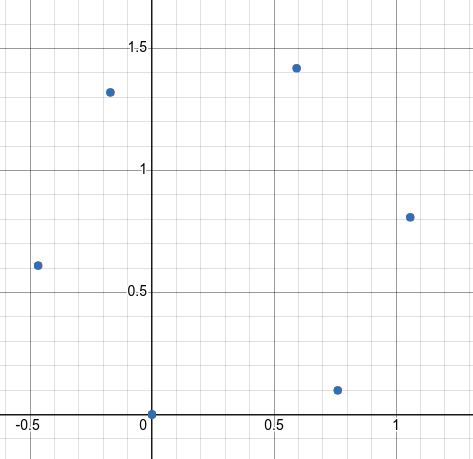
\includegraphics[width=.9\textwidth]{Figures/Lab\ Three/L3E-1}
  \caption{Both $S_{12}$ (\textcolor{red}{red}) and $S_{21}$ (\textcolor{blue}{blue}) Plotted}
  \label{fig:3}
\end{figure}

\begin{figure}[H]
  \centering
  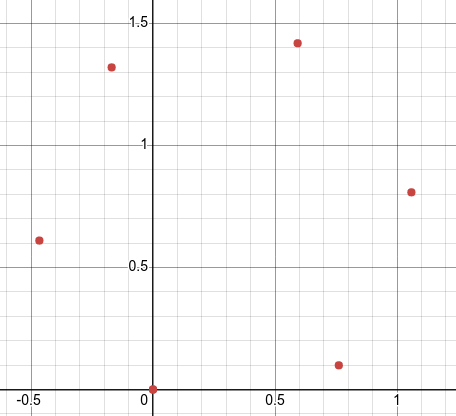
\includegraphics[width=.9\textwidth]{Figures/Lab\ Three/L3E-2}
  \caption{Only $S_{12}$ Plotted}
  \label{fig:4}
\end{figure}

We may see that the plots correspond to, more or less, circular shapes. Furthermore, it may be observed that, for each data point, $P_{12}\approx -P_{21}$, and $Q_{12}\approx -Q_{21}$, which is why it is difficult to see $S_{12}$ in Figure \ref{fig:3}. To more easily see $S_{12}$, it is plotted separately in Figure \ref{fig:4}.

\subsection{Part F: Using a Power Graphing Applet}

We now use a transmission line power graphing applet. This allows us to obtain a figure for each value of $\theta_2$, shown in Figures \ref{fig:5} to \ref{fig:11}:

\begin{figure}[H]
  \centering
  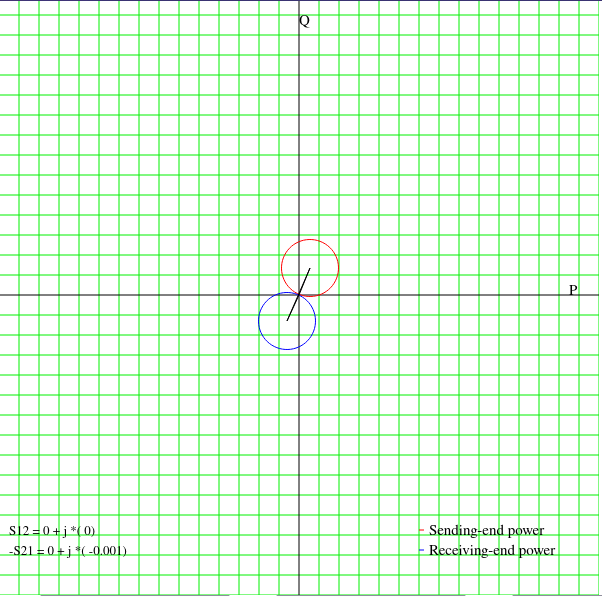
\includegraphics[width=.65\textwidth]{Figures/Lab\ Three/L3F-1}
  \caption{$\theta_2=0^{\circ}$}
  \label{fig:5}
\end{figure}

\begin{figure}[H]
  \centering
  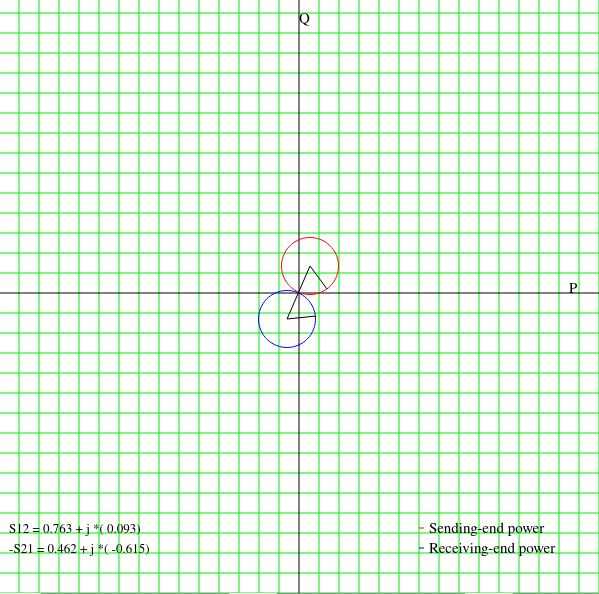
\includegraphics[width=.65\textwidth]{Figures/Lab\ Three/L3F-2}
  \caption{$\theta_2=-60^{\circ}$}
  \label{fig:6}
\end{figure}

\begin{figure}[H]
  \centering
  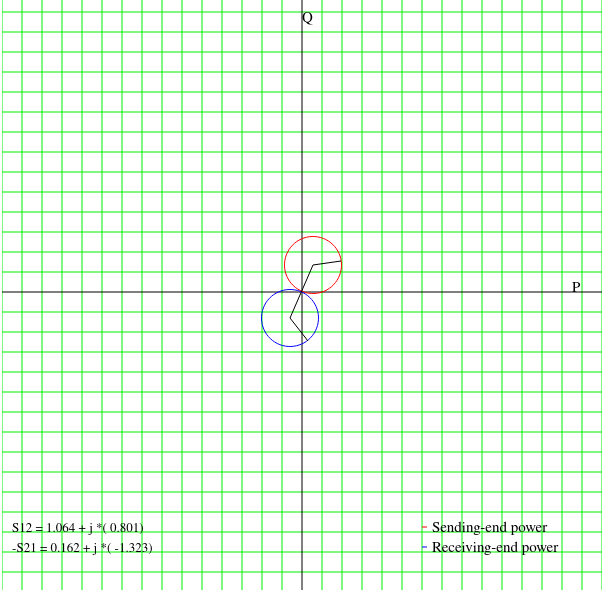
\includegraphics[width=.65\textwidth]{Figures/Lab\ Three/L3F-3}
  \caption{$\theta_2=-120^{\circ}$}
  \label{fig:7}
\end{figure}

\begin{figure}[H]
  \centering
  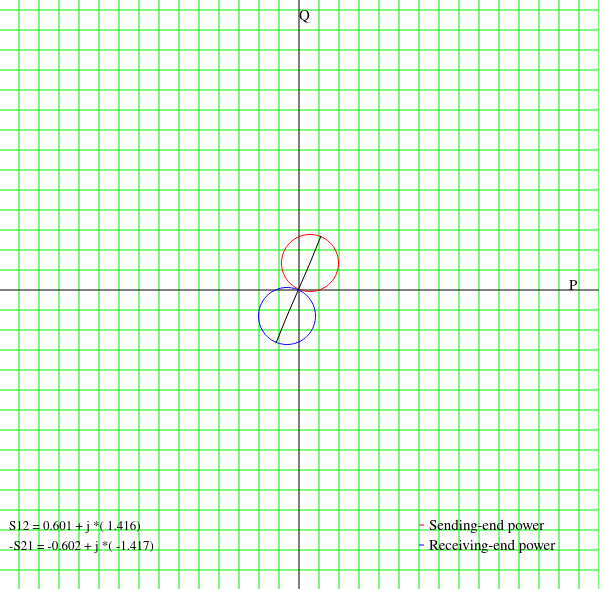
\includegraphics[width=.65\textwidth]{Figures/Lab\ Three/L3F-4}
  \caption{$\theta_2=-180^{\circ}$}
  \label{fig:8}
\end{figure}

\begin{figure}[H]
  \centering
  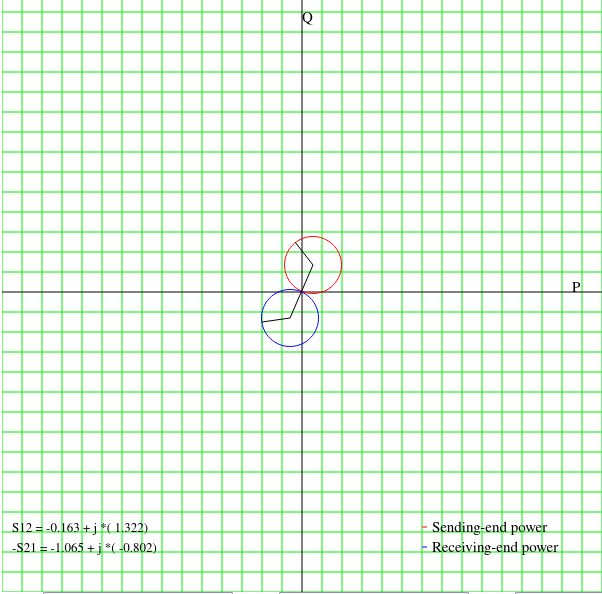
\includegraphics[width=.65\textwidth]{Figures/Lab\ Three/L3F-5}
  \caption{$\theta_2=-240^{\circ}$}
  \label{fig.65}
\end{figure}

\begin{figure}[H]
  \centering
  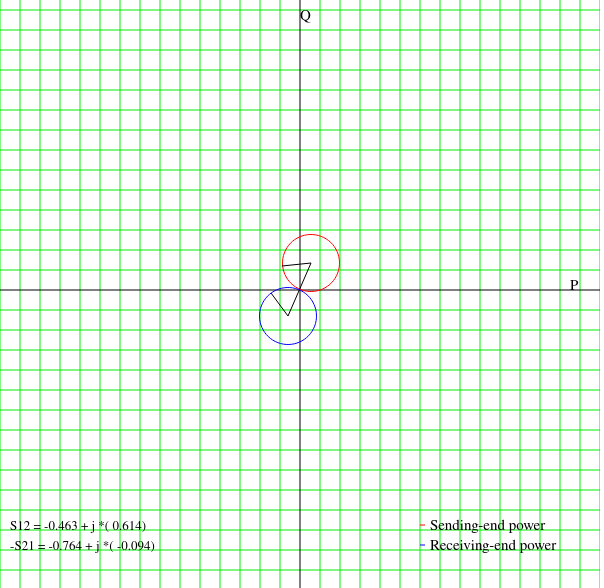
\includegraphics[width=.65\textwidth]{Figures/Lab\ Three/L3F-6}
  \caption{$\theta_2=-300^{\circ}$}
  \label{fig:10}
\end{figure}

\begin{figure}[H]
  \centering
  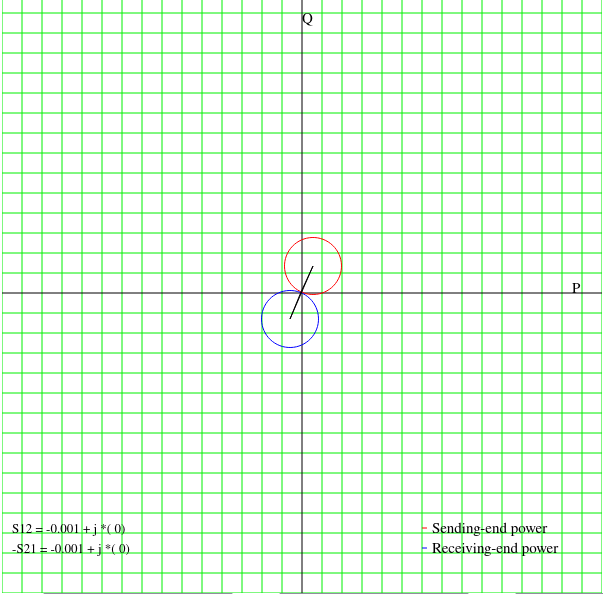
\includegraphics[width=.65\textwidth]{Figures/Lab\ Three/L3F-7}
  \caption{$\theta_2=-360^{\circ}$}
  \label{fig:11}
\end{figure}

From the plots above, we may observe that the points plotted in Figures \ref{fig:3} and \ref{fig:4} correspond to the points indicate by the radial lines. Furthermore, the red circle (sending end power), corresponds to a connection of the points plotted in Figures \ref{fig:3} and \ref{fig:4}.

\subsection{Part G: Analyzing the Effect of Voltage Magnitude}

Applying the given conditions ($\theta_2=20^{\circ}$ and $|V_2|=.8[p.u.]$), we may obtain the following figure:

\begin{figure}[H]
  \centering
  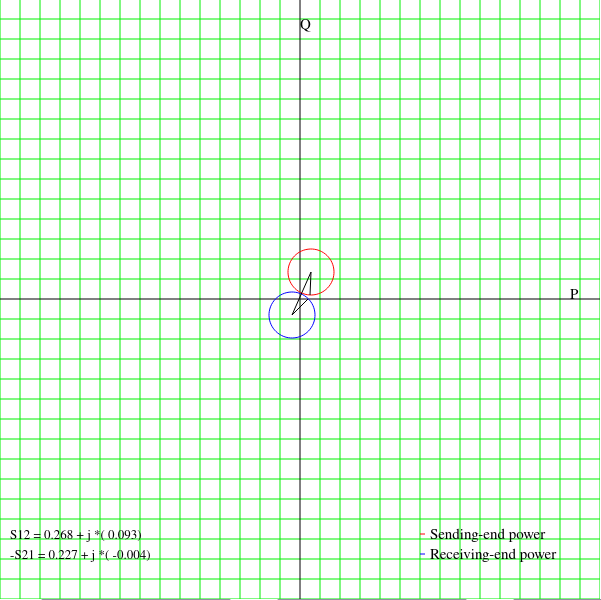
\includegraphics[width=.9\textwidth]{Figures/Lab\ Three/L3G}
  \caption{Plot Showing Decreased $V_2$ Magnitude}
  \label{fig:12}
\end{figure}

We may notice that, by decreasing the voltage magnitude at the receiving end, the magnitude of power effectively decreased for both ends. In the default case, we get $S_{12}=.26-.061j$ and $-S_{21}=.224-.146j$, while we get $S_{12}=.268+.93j$ and $-S_{21}=.227-.004j$ for the modified case. We can thus see that, although there is slightly more real power transmitted, more reactive power is consumed. This is exhibited by a shrinking of the radius of plotted circles.

\subsection{Part H: Changing $\theta_2$}

Changing $\theta_2$ from $-10[^{\circ}]$ to $-30[^{\circ}]$ gives us the following plots:

\begin{figure}[H]
  \centering
  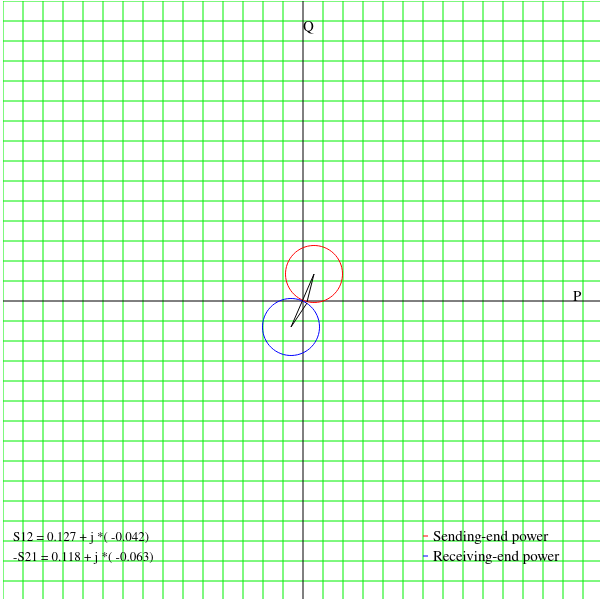
\includegraphics[width=.65\textwidth]{Figures/Lab\ Three/L3H-1}
  \caption{$\theta_2=-10[^{\circ}]$ Case}
  \label{fig:13}
\end{figure}

\begin{figure}[H]
  \centering
  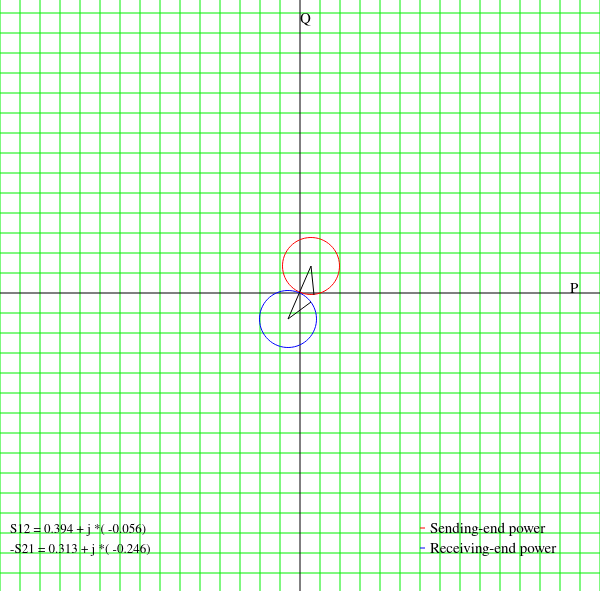
\includegraphics[width=.65\textwidth]{Figures/Lab\ Three/L3H-2}
  \caption{$\theta_2=-30[^{\circ}]$ Case}
  \label{fig:14}
\end{figure}

We may observe that, for the first case, the complex powers are: $S_{12}=.127-.042j$ and $-S_{21}=.118-.063j$. For the second case, they become: $S_{12}=.394-.056j$ and $-S_{21}=.313-.246j$. Thus, we see that increasing the phase angle difference drastically increased the magnitude of the complex power for both the receiving and sending end.

\section{Conclusion}

\begin{enumerate}

  \item We may observe that, when the magnitude of one of the voltages is decreased, the magnitude of the complex power decreases. That is, the radii of the circles shrink. Conversely, if the magnitude of one of the voltages is increased, the radii of the circles increase. Whichever magnitude voltage is changed has the circle remain centered at the same point, while the other circle moves according to the distance set by the line between their centers.

  \item We may notice that, the greater the voltage magnitudes, the greater the overall complex power output. Therefore, the components of the complex output also increase accordingly. The sending-end real power is maximized when the angle of the line impedance, $\alpha$ and the phase difference, $\theta_{12}=-\theta_2$ sum to $180[^{\circ}]$, such that $\alpha+\theta_{12}=\alpha-\theta_{2}=180[^{\circ}]$; this is minimized when $\alpha+\theta_{12}=\alpha-\theta_{2}=360=0[^{\circ}]$. The sending-end reactive power is maximized with a $90[^{\circ}]$ shift, or when $\alpha+\theta_{12}=\alpha-\theta_{2}=270[^{\circ}]$, and minimized when $\alpha+\theta_{12}=\alpha-\theta_{2}=90[^{\circ}]$. Conversely, receiving-end power maximization depends on the difference. The real power is maximized when $\alpha-\theta_{12}=\alpha+\theta_{2}=360=0[^{\circ}]$ and minimized when $\alpha-\theta_{12}=\alpha+\theta_{2}=180[^{\circ}]$. Similarly, the reactive power is maximized when $\alpha-\theta_{12}=\alpha+\theta_{2}=270[^{\circ}]$ and minimized when $\alpha-\theta_{12}=\alpha+\theta_{2}=90[^{\circ}]$.\\

\end{enumerate}

Throughout this experiment, we viewed the behavior of the transmission line model on power. By tweaking the phase difference, magnitude of voltages, and various capacitor configurations, we were able to reinforce topics regarding the model introduced in class.

\end{document}
